\documentclass[a4paper,11pt,dvipdfmx]{jsarticle}


% 数式
\usepackage{amsmath,amsfonts}
\usepackage{bm}

% 画像
\usepackage[dvipdfmx]{graphicx}
\usepackage{framed}

% 図形
\usepackage{tikz}
\usetikzlibrary{shapes.geometric}
\usetikzlibrary {shapes.misc}

% ソースコード
\usepackage{listings,jlisting,color}
\lstset{
language={Python},
backgroundcolor={\color[gray]{.85}},
basicstyle={\ttfamily},
identifierstyle={\small},
commentstyle={\small \color[rgb]{0,0.5,0}},
keywordstyle={\small\bfseries \color[rgb]{0.5,0,0.5}},
ndkeywordstyle={\small},
stringstyle={\small\ttfamily \color[rgb]{0,0,1}},
frame={tb},
breaklines=true,
columns=[l]{fullflexible},
numbers=left,
xrightmargin=0zw,
xleftmargin=3zw,
numberstyle={\scriptsize},
stepnumber=1,
numbersep=1zw,
lineskip=-0.5ex,
}
\renewcommand{\lstlistingname}{ソースコード}

\begin{document}
\begin{titlepage}
\noindent
\vspace{6cm}
\begin{center}
\begin{LARGE}
通信システム実験2 待ち行列シミュレーション
\end{LARGE}
\end{center}
\vspace{6cm}
\begin{flushright}
信州大学工学部 \
電子情報システム工学科 \
\begin{description}
\setlength{\leftskip}{8.9cm}
\item[  実験日:] 2023/11/01
\item[ 実験場所:] W2棟101室
\item[  実験者:] 21T2166D 渡辺 大樹
\item[共同実験者:] 20T2062A 斎藤 創真
\item[      ] 21T2004H 朝日 純菜
\item[      ] 21T2033A 岡村 椋平
\item[      ] 21T2091J 徳竹 稜平
\item[      ] 21T2099D 中田 奏音
\end{description}
\end{flushright}
\end{titlepage}

\definecolor{shadecolor}{gray}{0.70}


\section{実験内容}
本実験ではネットワークにおけるパケット通信のレスポンスなどに用いられる
待ち行列理論をバスの運行シミュレーションを通してその理論の体験、理解を進める目的で行う。

実験1ではベルヌーイ過程を、実験2では指数分布をシミュレーション、理解し、これらを用いて実験3でバスの運行シミュレーションを行う。

\section{レポート課題}
以下にレポート課題の解答を示す。

\subsection*{レポート課題1.1}
確率変数$Z$の分布関数$F_Z(x)$を密度関数$f_Z(x)$で表すと
\begin{align}
    F_Z(x) = \int_{-\infty}^{\infty}f_Z(x)dx
\end{align}
となる。

\subsection*{レポート課題1.2}
到着確率の期待値が$\frac{\delta}{p}$となることを示す。

タイムスロットの間隔を$\delta$,各スロットでの到着確率を$p$としたときの到着間隔の期待値を求める。
到着間隔の確率変数を$Z$,確率を$P_Z(n)$とすると$n=1,2,3,\cdots$に対して確率$P_Z(n)$は
\begin{equation}
    \begin{split}
        P_Z(1) &= p \\
        P_Z(2) &= p(1-p) \\
        P_Z(3) &= P(1-p)^2 
    \end{split}
\end{equation}
となる。
期待値の式は確率変数とその時の確率を掛け合わせ、
\begin{align}
    E[Z] = \sum_{n=1}^{\infty}n \cdot \delta \cdot P_Z(n) 
\end{align}
となる。

この式に先ほどの確率$P_Z(n)$の一般化した式を代入することで
\begin{align}
    E[Z] = \delta p\sum_{n=1}^{\infty}n(1-p)^{n-1}
\end{align}
という式が得られる。

ここでシグマの中身を部分和として計算していく。
\begin{align}
    S_n = \sum_{k=1}^{n}k(1-p)^{k-1}
\end{align}
とする。
$S_n$に$(1-p)$を掛け算すると
\begin{align}
    (1-p)S_n = \sum_{k=1}^{n}k(1-p)^k
\end{align}
となる。
(5)から(6)を引き算すると
\begin{align}
    pS_n = \sum_{k=1}^{n+1}(1-p)^{k-1}
\end{align}
という式が得られる。この式は初項$1$公比$(1-p)$の等比数列の和となるため
公式を用いて計算すると
\begin{align}
    pS_n = \frac{1-(1-p)^n}{p}
\end{align}
となる。すなわち$S_n$は
\begin{align}
    S_n = \frac{1-(1-p)^n}{p^2}
\end{align}
となる。

$S_n$は部分和のためnについて極限をとることで
\begin{align}
    \sum_{n=1}^{\infty}n(1-p)^{n-1} = \frac{1}{p^2}
\end{align}
となる。これを(4)式に代入しなおすことで
\begin{align}
    E[Z] = \frac{\delta}{p}
\end{align}
が得られる。これにより題意は示された。

\subsection*{レポート課題1.3}
10面サイコロの0-9の目をすべて出すために必要なサイコロを振る回数の平均を求める。

サイコロの目をコンプリートする回数を計算することは上記課題1.2で行った
タイムスロットの到着間隔の期待値を考えることと同じで、k個目のサイコロの目がm回目で揃う確率は
$(\frac{k}{10})(1-\frac{k}{10})^{m-1}$となる。
これをmが無限大になるまで和を求めればよいためサイコロを振る回数の平均$E$は
\begin{align}
    E &= \sum_{k=1}^{10}\frac{1}{1-\frac{k}{10}}\\
      &= 10(\frac{1}{10}+\frac{2}{10}+\frac{3}{10}+\cdots+1)
\end{align}
となりしたがっておおよそ$E=29.28$という値が得られる。

\subsection{レポート課題2.1}
指数分布の密度関数が$f(x)=\lambda e^{-\lambda x}$であることを用いて
分布関数が$F(x)=1-e^{-\lambda x}$となることを示す。

密度関数を定義されるすべての$x$で積分することで分布関数が求まるので計算をすると
\begin{align}
    F(x) &= \int_{0}^{x}\lambda e^{-\lambda t}dt \\
         &= \left[-e^{-\lambda t}\right]_{0}^{x} \\
         &= 1 - e^{-\lambda x}
\end{align}
となり、よって題意は求まった。

\subsection{レポート課題2.2}
期待値は確率とそのときの値を掛け合わせたものび総和で求まる。指数分布は連続な確率関数なので
\begin{align}
    E[x] &= \int_{0}^{\infty}x(\lambda e^{-\lambda x})dx \\
         &= \left[xe^{-\lambda x}\right]_{0}^{\infty} - \lambda \int_{0}^{\infty} -\frac{1}{\lambda} e^{-\lambda x} dx \\
         &= -\frac{1}{\lambda} \left[e^{-\lambda x}\right]_{0}^{\infty} \\
         &= \frac{1}{\lambda}
\end{align}
と部分積分などを用いることで求まった。

\subsection{レポート課題2.3}
ここでは分布関数$F(x)=1-e^{-\lambda x}$の逆関数が$F^{-1}(x)=-\frac{1}{\lambda}\log(1-x)$
となることを示す。
\begin{align}
    y &= F(x) \\
      &= 1-e^{-\lambda x}
\end{align}
とする。$x$と$y$を入れ替えることで逆関数となる。入れ替えた後の関数を$y$について解いていく。
\begin{align}
    x &= 1 - e^{-\lambda y} \\
    e^{-\lambda y}  &= 1 - x \\
    -\lambda y &= \log(1-x) \\
    y &= -\frac{1}{\lambda}\log(1-x)
\end{align}
このように式を変形させることで示される。


\section{実験}
以下に実験とその結果について示していく。

\subsection{実験1}
実験1では、間隔$\delta$により短く区切られた一つのタイムスロットでそれぞれ確率$p$の確率的施行
を行い、成功か失敗かを決める、ベルヌーイ過程を実験的に行う。

今回の実験では$\delta=1,p=0.1$として計算をおこなう。この施行ののち、到着まで
いくつのタイムスロットで失敗をしたのかの到着間隔をヒストグラムにまとめる。

実験にはPythonを用いて発生させた乱数が0.1より小さいときに成功、大きいと失敗とし失敗した場合はまた同じ
施行を繰り返させ、施行が失敗した回数を数えることでそれを到着間隔とした。

用いたコードは以下ソースコード\ref{bern}に示す。
\lstinputlisting[language=python,caption=Beenoulli.py, label=bern]{C:/Program_Code/Python/CSE2/Bernoulli.py}

このコードによって得られたヒストグラムを図\ref{berhist}に示す.
\begin{figure}[h]
\centering
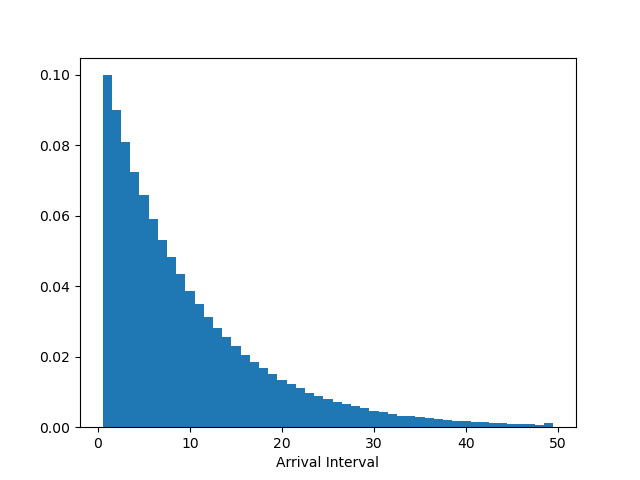
\includegraphics[width=80mm]{Bernoulli.png}
\caption{到着間隔の相対度数分布}
\label{berhist}
\end{figure}

この図\ref{berhist}が到着間隔の実験的な分布となる。

\subsection{実験2}
実験2では指数分布に従う乱数を実験的に発生させ、その累積相対度数のヒストグラムと平均値を
求め、指数分布の分布関数や期待値と比較していく。

一様乱数から任意の分布に従う確率変数を生成するには、今必要としている確率変数の分布関数を
$y=F(x)$,$[0,1)$の一様乱数を$U$としたとき
\begin{equation}
    X=F^{-1}(U)
\end{equation}
を計算すればよい。

レポート課題2.3で示した内容を用いれば、指数分布を一様乱数から生成するための式は
\begin{equation}
    X = -\frac{1}{\lambda}\log(1-U)
\end{equation}
となる。
この式から得られた乱数を統計的に処理して累積相対度数のグラフと平均値を取得する。

用いたコードは以下ソースコード\ref{expo}に示す。
\lstinputlisting[language=python,caption=Exporand.py, label=expo]{C:/Program_Code/Python/CSE2/Exporand.py}

このコードで得られたヒストグラムを図\ref{expohist}に示す。
\begin{figure}[h]
\centering
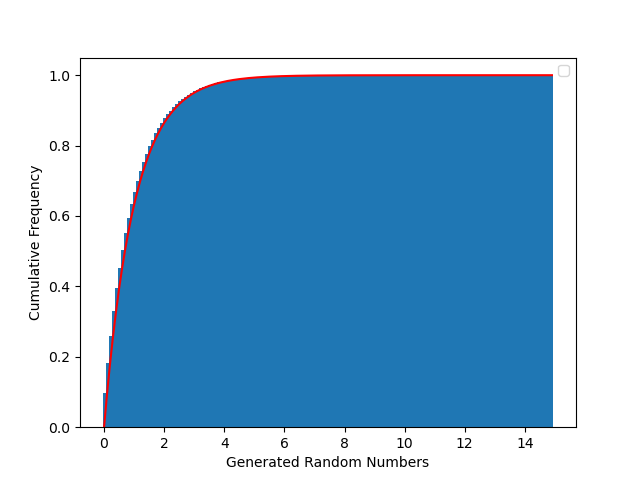
\includegraphics[width=80mm]{Exporand.png}
\caption{指数分布に従う乱数の累積相対度数と指数分布の分布関数}
\label{expohist}
\end{figure}

図\ref{expohist}では青色のヒストグラムが実験で発生させた乱数の累積グラフ、
赤色のグラフが指数分布の分布関数になっている。どちらともパラメータ$\lambda$は$1$で計算している。
ここからわかるように、ほとんど一致したグラフを生成できていることがわかる。

またこの施行で得られた平均値は0.999425708871489となった。
期待値は$\frac{1}{\lambda}$であることから$\lambda=1$であるとき期待値も$1$となるため、
そこそこの精度で一致していることが読み取れる。


\end{document}